\documentclass[utf8x]{beamer}

\mode<presentation>
{
  \usetheme{Warsaw}

  %\setbeamercovered{transparent}
}


\usepackage[english]{babel}

\usepackage[utf8x]{inputenc}

\usepackage{times}
\usepackage[T1]{fontenc}

\title[Back to the Future in one Week]
{%
    Back to the Future in one Week — Implementing a Smalltalk VM in PyPy%
}

\author[Bolz, Kuhn, Lienhard, Matsakis, Nierstrasz, Renggli, Rigo, Verwaest]
{
    \textcolor{green!50!black}{Carl~Friedrich~Bolz}\inst{1} \and
    \textcolor{green!50!black}{Adrian~Kuhn\inst{2}} \and
    Adrian~Lienhard\inst{2} \and
    Nicholas~D.~Matsakis\inst{3} \and
    Oscar~Nierstrasz\inst{2} \and
    Lukas~Renggli\inst{2} \and
    Armin~Rigo \and
    \textcolor{green!50!black}{Toon~Verwaest}\inst{2}
}

\institute[Bern and others]
{
    \inst{2}%
    Software Composition Group\\ University of Bern, Switzerland
    \and%
    \vskip-2mm
    \inst{1}
    Softwaretechnik und Programmiersprachen\\ Heinrich-Heine-Universit\"at D\"usseldorf
    \and%
    \vskip-2mm
    \inst{3}%
    ETH Zürich, Switzerland
}


\date{Squeak e.V. Meeting, May 17 2008 \\
(presented at S3)
}


% Delete this, if you do not want the table of contents to pop up at
% the beginning of each subsection:
%\AtBeginSubsection[]
%{
%  \begin{frame}<beamer>
%    \frametitle{Outline}
%    \tableofcontents[currentsection,currentsubsection]
%  \end{frame}
%}


% If you wish to uncover everything in a step-wise fashion, uncomment
% the following command: 

%\beamerdefaultoverlayspecification{<+->}


\begin{document}

\begin{frame}
  \titlepage
\end{frame}

%\begin{frame}
%  \frametitle{Outline}
%  \tableofcontents
  % You might wish to add the option [pausesections]
%\end{frame}

\begin{frame}
    \frametitle{Scope}
    This demo is about:
    \begin{itemize}
    \item writing a Squeak implementation (called "SPy") in Python
    \item with eight people
    \item in five days
    \item using PyPy
    \end{itemize}
\end{frame}

\begin{frame}
    \frametitle{What is PyPy?}
    \begin{itemize}
    \item started as a Python implementation in Python
    \item Open Source project, MIT license
    \item developed into a general environment for implementing dynamic languages
    \item supports the language developer with a lot of infrastructure
    \item most important goal: abstracting over low-level details
    \item don't fix decisions about low-level details early
    \end{itemize}
\end{frame}

\frame[plain]{
    \frametitle{What is PyPy?}
    \centering
    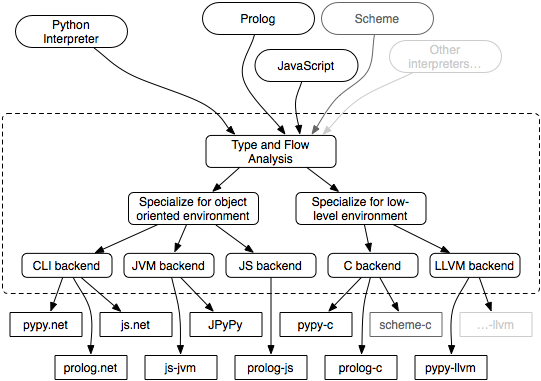
\includegraphics[height=8cm]{dynlang}
}
\begin{frame}
    \frametitle{The SPy VM}
    \begin{itemize}
        \item complete but simple, straight-forward Squeak interpreter in RPython
        \item goal is to fully support loading and running Squeak images
        \item source code essentially free of low-level details, no GC
        \item written during a five-day sprint in October in Bern
    \end{itemize}
\end{frame}

\begin{frame}
    \frametitle{Current Status}
    \begin{itemize}
    \item bytecodes fully implemented
    \item many primitives implemented: arithmetic primitives, object primitives
    \item can load Squeak images (both 2.0 and 3.9)
    \item runs tiny benchmarks
    \item runs arbitrary code
    \item resume image
    \end{itemize}
    \pause
    Open Issues:
    \begin{itemize}
    \item any I/O
    \item graphics
    \item performance
    \item \#someInstance, \#nextInstance
    \item \#become
    \item tests for threading and exceptions
    \end{itemize}
\end{frame}

\frame[containsverbatim, plain, shrink=10]{
  \begin{verbatim}
  primitiveSquareRoot
    | rcvr |
    self var: #rcvr type: 'double '.
    rcvr := self popFloat.
    self success: rcvr >= 0.0.
    successFlag
        ifTrue: [self pushFloat:
            (self cCode: 'sqrt(rcvr)'
                  inSmalltalk: [rcvr sqrt])]
        ifFalse: [self unPop: 1]









  \end{verbatim}
}


\frame[containsverbatim, plain, shrink=10]{
  \begin{verbatim}
  primitiveSquareRoot
    | rcvr |
    self var: #rcvr type: 'double '.
    rcvr := self popFloat.
    self success: rcvr >= 0.0.
    successFlag
        ifTrue: [self pushFloat:
            (self cCode: 'sqrt(rcvr)'
                  inSmalltalk: [rcvr sqrt])]
        ifFalse: [self unPop: 1]


  @expose_primitive(FLOAT_SQUARE_ROOT,
                    unwrap_spec=[float])
def func(interp, f): 
    if f < 0.0:
        raise PrimitiveFailedError
    w_res = utility.wrap_float(math.sqrt(f))
    return w_res
  \end{verbatim}
}

\frame[plain]{
    \frametitle{Performance (tiny Benchmark)}
    \centering
    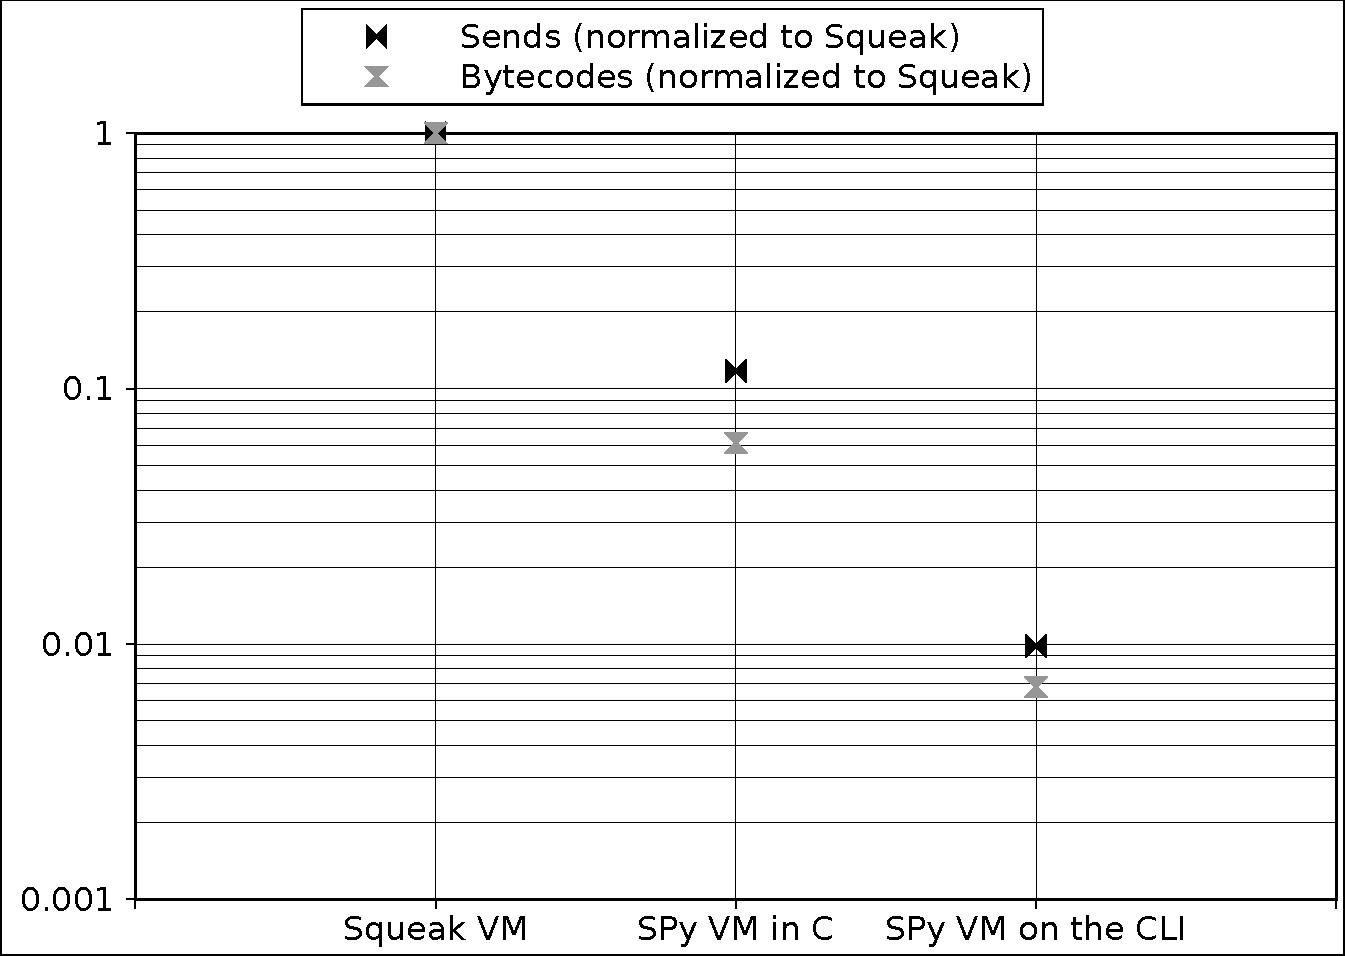
\includegraphics[height=8cm]{speed}
}

\begin{frame}
    \frametitle{Results}
    {\bf Good Points of the Approach:}
    \begin{itemize}
    \item simple, understandable, high-level Squeak implementation
    \item mostly free of low-level details: no GC, no manual pointer tagging
    \item written in a short amount of time
    \item runs on various platforms
    \item extensible tool chain
    \end{itemize}
    \pause
    {\bf Bad Points of the Approach:}
    \begin{itemize}
    \item not really fast (yet)
    \item RPython isn't Python
    \end{itemize}
\end{frame}

\begin{frame}
    \frametitle{Outlook}
    \begin{itemize}
    \item do graphical builtins, to actually start the full environment
    \item Squeak-specific optimizations:
    \item method-cache (should be easy with shadows)
    \item JIT
    \item lessons learned for a "SqueaSquea"?
    \end{itemize}
  \begin{block}{
    Join the Sprint!}
    \bigskip
    \hskip 1cm Saturday - Thursday, C-Base Berlin
    \bigskip
  \end{block}
\end{frame}

\end{document}
